%%***( Resumen )********************************************************************

Para las personas que se dedican a la investigación de animales les resulta complicado hacer salidas de campo para la toma de información, ya que esto representa un problema para la precisión de la información y de su presencia asociada al entorno natural de los animales. Es por eso que se presenta un proyecto que diseña un sistema para la toma de información de animales por medio de dispositivos electrónicos, cuya información es transmitida y almacenada en la nube,.

Este proyecto busca mostrar el funcionamiento de dicho sistema, considerando como usuarios finales investigadores y personas interesadas en la información recolectada en una zona específica en el contexto Colombiano, dicha información es obtenida por medio del uso de internet para la transmisión de datos y su recolección.

%%==================================================================================
\section{Resumen ejecutivo}

Como se conoce, los investigadores se encargan de estudiar muchas características de los animales, es por eso que es necesario definir que características específicas se puede extraer de los animales, para ello se pretenden extraer datos como:

\begin{itemize}
    \item Imagen de los animales.
    \item Fecha de la captura de los datos.
    \item Grabaciones de los animales.
    \item Audio de los sonidos emitidos por los animales y el entorno.
\end{itemize}

Para la recolección de esta información se pretende utilizar los siguientes dispositivos electrónicos: \emph{Cámaras de Vídeo}, \emph{Micrófonos} y \emph{Sensores de Movimiento}. Algo importante que se debe aclarar de todo esto es que los dispositivos de la toma de datos estarán conectados a un controlador, dicho controlador emitirá y recibirá información por medio de internet hacia y de un servidor que funciona en lo que se conoce como nube, en donde se almacenará la información en una base de datos de forma periódica. Por último, los usuarios finales (como investigadores) pueden acceder a esta información por medio de una aplicación en un dispositivo de cómputo, ingresando parámetros o rangos para filtrar la información si lo desean.

%%==================================================================================
\section{Glosario}

Algunos términos que se deben definir dentro del contexto del proyecto son:

\begin{itemize}
    \item \textbf{Nube:} es una red enorme de servidores remotos, conectada a través de internet, que funciona cómo un único ecosistema. Están diseñados para almacenar y administrar datos, ejecutar aplicaciones o entregar contenido.
    \item \textbf{Controlador:} es un circuito o componente electrónico utilizado para controlar otro circuito o componente electrónico.
\end{itemize}

%%==================================================================================
\section{El equipo de diseño}

El equipo de diseño y trabajo se compone de los siguientes integrantes:

\begin{figure}[h]
    \centering
    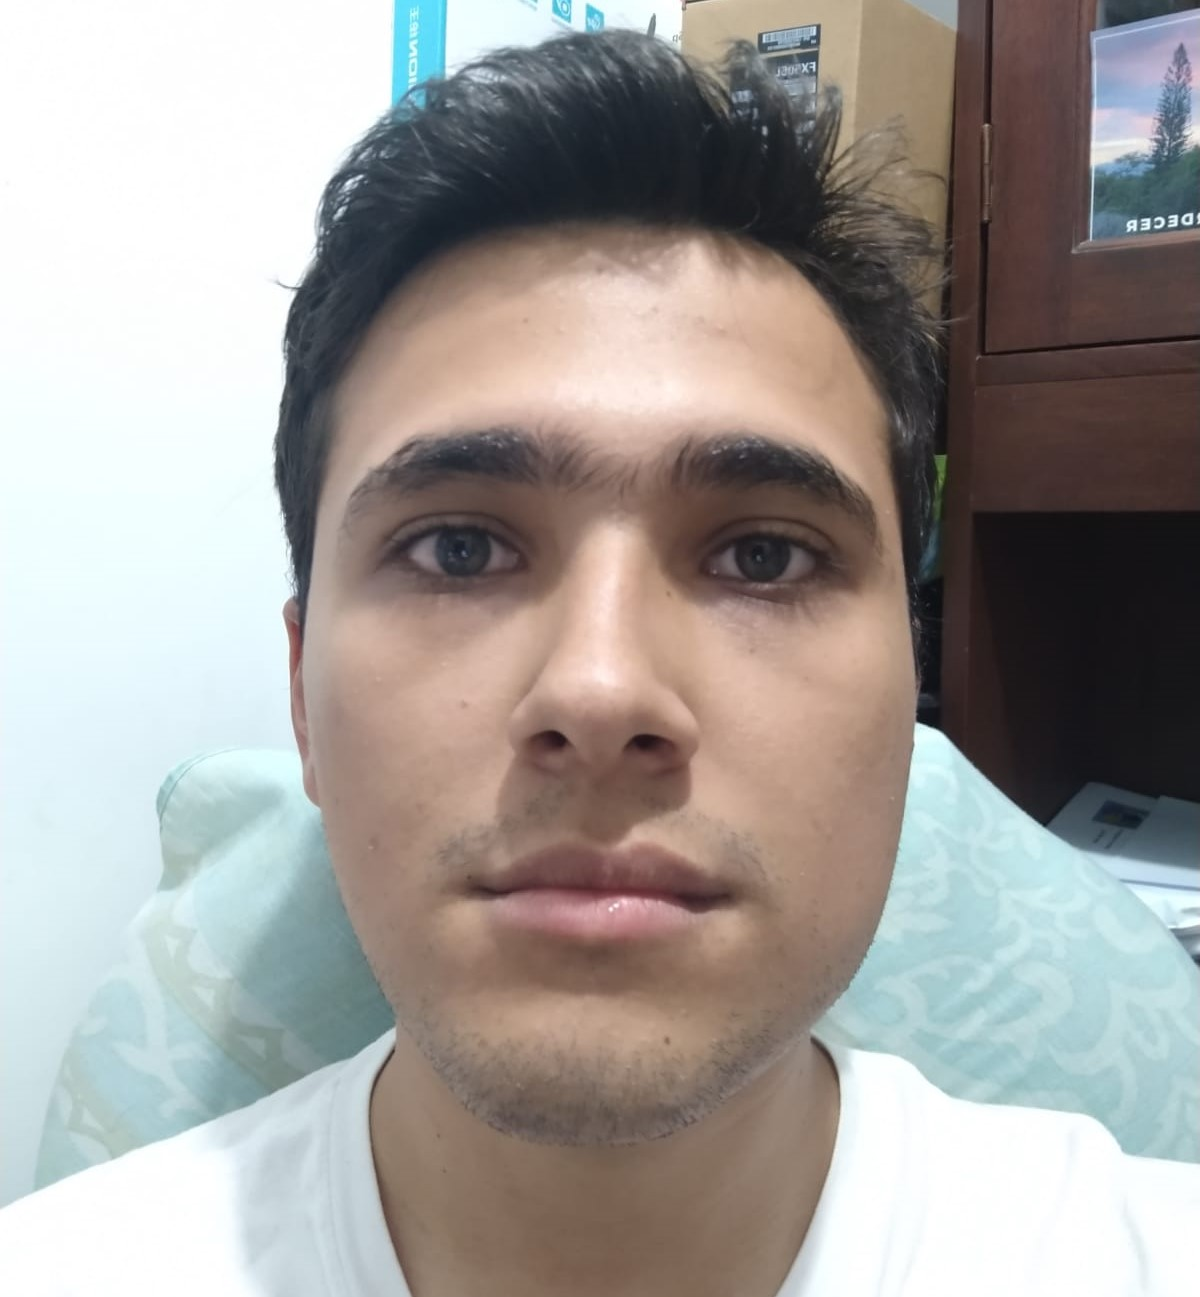
\includegraphics[width=0.50\textwidth]{images/Luis.jpeg}
    \caption{Luis Alberto Salazar. Estudiante de Ingeniería en Sistemas.}
    \label{Luis}
\end{figure}

Luis, se ve a él mismo como una persona responsable con sus proyectos y sueños, considera que su valor más importante que lo caracteriza es la empatía. Uno de sus más grandes rasgos es la capacidad de liderar a las personas en cualquier proyecto o situación, pues siempre buscar ayudar a las personas a alcanzar un objetivo en común. Se considera disciplinado y perseverante para llevar a cabo sus metas y proyectos.

\begin{figure}[h]
    \centering
    
\includegraphics[width=0.50\textwidth]{images/Dilan.jpeg}
    \caption{Dilan Andrés Correa. Estudiante de Ingeniería en Sistemas.}
    \label{Dilan}
\end{figure}

Dilan, es un estudiante que nunca se rinde para realizar sus tareas, se ve a él mismo como una persona que se esfuerza por lo que hace y la empatía hacia los demás. El siempre busca el bienestar de las personas, pues en sus aportes trata de analizar el menor impacto para los demás. Se considera como una persona que ve más allá de los problemas y siempre busca solucionar los dilemas que se le presentan, le gusta escuchar y entender lo que dicen los demás. Se considera buen compañero para trabajar en equipo.

\pagebreak

\begin{figure}[h]
    \centering
    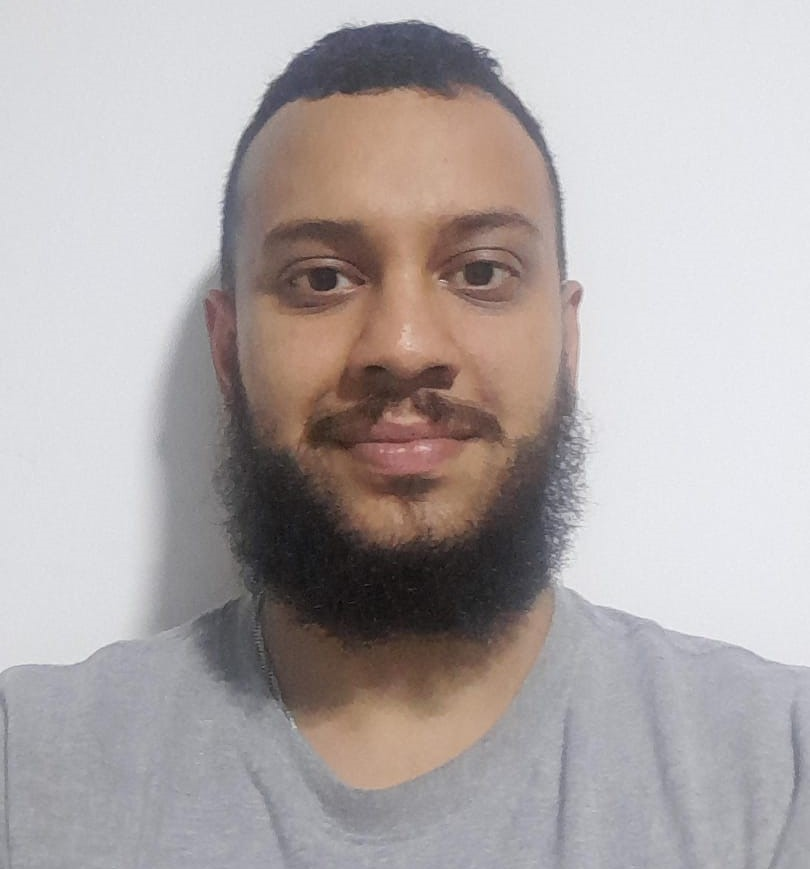
\includegraphics[width=0.50\textwidth]{images/Guido.jpeg}
    \caption{Guido Ernesto Salazar. Estudiante de Ingeniería en Sistemas.}
    \label{Guido}
\end{figure}

Guido, se considera a si mismo como una persona tranquila y crítica de muchas cosas que él ve. Siente que ve más allá de las cosas y se considera como una persona analítica de todas las situaciones que tiene en su vida. Es una persona responsable y comprometida con lo que hace, busca siempre hacer la mejor solución y considerar todos los casos posibles, le encanta resolver problemas y retarse buscando soluciones que sea eficientes y que solucionen en su totalidad el problema, la mejor solución.

